\documentclass[12pt]{article}

\usepackage{fullpage}
\usepackage{mdframed}
\usepackage{colonequals}
\usepackage{algpseudocode}
\usepackage{algorithm}
\usepackage{tcolorbox}
\usepackage[all]{xy}
\usepackage{proof}
\usepackage{mathtools}
\usepackage{bbm}
\usepackage{amssymb}
\usepackage{amsthm}
\usepackage{amsmath}
\usepackage{amsxtra}
\newcommand{\bb}{\mathbb}


\newtheorem{theorem}{Theorem}[section]
\newtheorem{corollary}{Corollary}[theorem]
\newtheorem{lemma}{Lemma}

\newcommand{\mathcat}[1]{\textup{\textbf{\textsf{#1}}}} % for defined terms

\newenvironment{problem}[1]
{\begin{tcolorbox}\noindent\textbf{Problem #1}.}
{\vskip 6pt \end{tcolorbox}}

\newenvironment{enumalph}
{\begin{enumerate}\renewcommand{\labelenumi}{\textnormal{(\alph{enumi})}}}
{\end{enumerate}}

\newenvironment{enumroman}
{\begin{enumerate}\renewcommand{\labelenumi}{\textnormal{(\roman{enumi})}}}
{\end{enumerate}}

\newcommand{\defi}[1]{\textsf{#1}} % for defined terms

\theoremstyle{remark}
\newtheorem*{solution}{Solution}

\setlength{\hfuzz}{4pt}

\newcommand{\calC}{\mathcal{C}}
\newcommand{\calF}{\mathcal{F}}
\newcommand{\C}{\mathbb C}
\newcommand{\N}{\mathbb N}
\newcommand{\Q}{\mathbb Q}
\newcommand{\R}{\mathbb R}
\newcommand{\Z}{\mathbb Z}
\newcommand{\br}{\mathbf{r}}
\newcommand{\RP}{\mathbb{RP}}
\newcommand{\CP}{\mathbb{CP}}
\newcommand{\nbit}[1]{\{0, 1\}^{#1}}
\newcommand{\bits}{\{0, 1\}^{n}}
\newcommand{\bbni}{\bigbreak \noindent}
\newcommand{\norm}[1]{\left\vert\left\vert#1\right\vert\right\vert}

\let\1\relax
\newcommand{\1}{\mathbf{1}}
\newcommand{\fr}[2]{\left(\frac{#1}{#2}\right)}

\newcommand{\vecz}{\mathbf{z}}
\newcommand{\vecr}{\mathbf{r}}
\DeclareMathOperator{\Cinf}{C^{\infty}}
\DeclareMathOperator{\Id}{Id}

\DeclareMathOperator{\Alt}{Alt}
\DeclareMathOperator{\ann}{ann}
\DeclareMathOperator{\codim}{codim}
\DeclareMathOperator{\End}{End}
\DeclareMathOperator{\Hom}{Hom}
\DeclareMathOperator{\id}{id}
\DeclareMathOperator{\M}{M}
\DeclareMathOperator{\Mat}{Mat}
\DeclareMathOperator{\Ob}{Ob}
\DeclareMathOperator{\opchar}{char}
\DeclareMathOperator{\opspan}{span}
\DeclareMathOperator{\rk}{rk}
\DeclareMathOperator{\sgn}{sgn}
\DeclareMathOperator{\Sym}{Sym}
\DeclareMathOperator{\tr}{tr}
\DeclareMathOperator{\img}{img}
\DeclareMathOperator{\CandE}{CandE}
\DeclareMathOperator{\CandO}{CandO}
\DeclareMathOperator{\argmax}{argmax}
\DeclareMathOperator{\first}{first}
\DeclareMathOperator{\last}{last}
\DeclareMathOperator{\cost}{cost}
\DeclareMathOperator{\dist}{dist}
\DeclareMathOperator{\path}{path}
\DeclareMathOperator{\parent}{parent}
\DeclareMathOperator{\argmin}{argmin}
\DeclareMathOperator{\excess}{excess}
\let\Pr\relax
\DeclareMathOperator{\Pr}{\mathbf{Pr}}
\DeclareMathOperator{\Exp}{\mathbb{E}}
\DeclareMathOperator{\Var}{\mathbf{Var}}
\let\limsup\relax
\DeclareMathOperator{\limsup}{limsup}
%Paired Delims
\DeclarePairedDelimiter\ceil{\lceil}{\rceil}
\DeclarePairedDelimiter\floor{\lfloor}{ \rfloor}


\newcommand{\dagstar}{*}

\newcommand{\tbigwedge}{{\textstyle{\bigwedge}}}
\setlength{\parindent}{0pt}
\setlength{\parskip}{5pt}


\begin{document}

\title{CS 40: Computational Complexity}

\author{Sair Shaikh}
\maketitle

% Collaboration Notice: Talked to Henry Scheible '26 to discuss ideas.



\begin{problem}{1}
    Compute the fundamental group of the complement of $k \geq 1$ points in the orientable surface $M_g$ of genus $g$.
\end{problem}
\begin{solution}
    The orientable surface $M_g$ of genus $g$ can be realized as a $4g$-gon with pairs of edges identified becoming a $\bigwedge^{2g} S^1$, glued along the boundary with a disk. Let $x_0$ be the vertex of the polygon (all vertices are identified together).The fundamental group of $M_g$ is given by the presentation:
    \[
        \pi_1(M_g, x_0) = \langle a_1, b_1, \ldots, a_g, b_g \mid [a_1, b_1]\cdots[a_g, b_g] \rangle
    \]  
    We puncture this at $k$ points in the interior of the polygon to get our space. \bbni  
    Let $x_0$ be the vertex of the CW complex. Draw $\alpha_1, \cdots, \alpha_k-1$ around $k-1$ of the holes. Each of these loops bounds a disk with a single hole, that can be contracted to this loop. The remaining center of the polygon is a $2$-cell with one hole that can be contracted to the boundary. Notably, this removes the $2$-cell and all the relations on the generators of the fundamental group. Thus, we have $2g$ free generators $a_1, b_1, \cdots, a_g, b_g$ and $k-1$ additional generators $\alpha_1, \cdots, \alpha_k$ corresponding to the loops around the punctures. Thus, we get the free group on $2g+k-1$ generators. 
\end{solution}
\newpage 

\begin{problem}{2}
    In the orientable surface $M_g$ of genus $g$, let $C$ be a circle that separates $M_g$ into two compact subsurfaces $M_h'$ and $M_k'$ obtained from the closed surfaces $M_h$ and $M_k$ by deleting an open disk from each. Show that $M'_h$ does not retract onto its boundary circle $C$, and hence $M_g$ does not retract onto $C$. (\emph{Hint:} abelianize $\pi_1$.) On the other hand, show that $M_g$ does retract onto the nonseparating circle $C'$ in the figure. 
    \begin{center}
        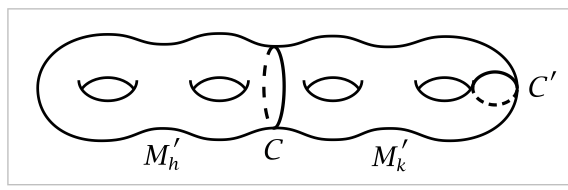
\includegraphics{HW5Image.png}
    \end{center}
\end{problem}
\begin{solution}
    Note that $M_h'$ is equivalent to a disk removed from $M_h$. In the CW complex picture, $M_h$ looks like $\bigwedge^2h S^1$, with a $2$-cell attached along the boundary. Puncturing $M_h$ involves puncturing the $2$-cell, which then deformation retracts to its boundary, $\bigwedge^{2h} S^1$ and thus has fundamental group: 
    \[ \pi_1(M_h') = \langle a_1, b_1\cdots, a_h, b_h \rangle \]
    The abelianization of this is $\Z^{2h}$. If there existed a retraction $r: M_h' \to C$, then we would have $\iota_*: \pi_1(C) \to \pi_1(M_h')$ injective (as $r_* \circ \iota_* = \id_{\pi_1(C)}$). Thus, as abelianization is a functor, we induce: 
    \[ \iota_*^{ab}: \Z \to \Z^{2h} \]
    Since $\Z$ is abelian, this map must also be injective (as the image of $\iota_*$ was abelian to begin with). However, note that the generator of $\pi_1(C)$ is mapped by $\iota_*$ to the commutator $[a_1, b_1]\cdots [a_h, b_h]$ in $\pi_1(M_h')$ (as we can easily see from the CW complex picture). In the abelianization, this is trivial, thus $\iota_*^{ab}$ is the trivial map, which is not injective. This is a contradiction. Thus, $M_h'$ does not retract onto $C$. This implies that $M_g$ does not retract onto $C$ as restricting this would give a retraction of $M_h'$ onto $C$. \bbni
    However, consider a non-separating circle $C'$. Note that the CW complex picture of $M_g$ is a $4g$-gon (cyclically $a_1 \cdot b_1 \cdot a_1^{-1} \cdot b_1^{-1} \cdot a_2 \cdot  \ldots \cdot b_n^{-1} a_1$) with pairs of edges identified. We can identify $C'$ with one of the $1$-cells, $a_1$, on the boundary. Note next that we can retract the CW complex onto the line joining the end of $b^{-1}$ to the start of $a_1$, and then retract this further to the identify the end of $b^{-1}$ with the start of $a_1$. This trivially does not violate any of the edge identifications on the $4g$-gon. Then, we are left with a square with opposite edges identified (a torus). We can vertically project this square down to $a$ (this does not violate any identifications, as identified points on $a$ go to their counterparts, whereas for $b$ they just retract to a single identified point on both ends of $a$). Thus, we have obtained a retraction from $M_g$ to $C'$.
\end{solution}
\newpage 


\begin{problem}{3}
    Suppose that we construct a space $M$ from gluing two copies of the solid torus $S^1 \times D^2$ along their boundary tori by a map $f: S^1 \times S^1 \to S^1 \times S^1$. Compute $\pi_1(M)$ when
    \begin{enumerate}
    \item $f$ is the identity map.
    \item $f$ swaps the two circles, that is, $f(x,y) = (y,x)$. 
    \end{enumerate}
\end{problem}
\begin{solution}
    This can be done using CW-complexes, however, I will attempt to do this via Seifert Van Kampen since that appears clearer to me. \\
    Let $X$ be the whole space. Let $U$ be the first solid torus together with a contractible neighborhood of the second. Let $V$ be the second solid torus together with a contractible neighborhood of the first. Then $U \cap V$ is the identified boundary of the two solid tori, alongside contractible neighborhoods of both tori, which is path-connected. Clearly, $U$ and $V$ are open, $X = U \cup V$. Thus, we can apply Seifert Van Kampen Theorem. \bbni
    Note $U$ and $V$ are contractible to solid tori. Then, $\pi_1(U) = \langle a \rangle$ and $\pi_2(V) = \langle b \rangle$, where $a$ and $b$ are loops that go around the (not filled in) $S^1$ of the two solid tori respectively. Thus, we have that: 
    \[ \pi_1(X) = \langle a, b \rangle / N\]
    where $N$ is the normal subgroup generated by identifying pushforwards of the generators of $U \cap V$, which depends on the map $f$. Let $\alpha$ and $\beta$ be these generators for $\pi_1(U \cap V) = \pi_1(S^1 \times S^1)$, going around longitudinally and around the meridian. Then we have the following cases:
    \begin{enumerate}
        \item Let $f$ be the identity map, then the pushforward of $\alpha$ using the inclusions goes along the meridian of both solid tori $U$ and $V$ and the pushforward of $\beta$ goes along the longitude of both solid tori. Thus, one of these is the boundary of a disk in both $U$ and $V$, hence trivial, while the other maps to $a$ and $b$ in $U$ and $V$ respectively. Thus, 
        \[ N = \langle ab^{-1}\rangle \] 
        Thus, we have that:
        \[ \pi_1(X) = \langle a, b \mid ab^{-1} \rangle = \langle a \rangle \]
        \item Let $f$ be the map that swaps the two circles. Then the pushforward of $\alpha$ using the inclusions goes along the meridian of $U$ and the longitude of $V$, while the pushforward of $\beta$ goes along the longitude of $V$ and the meridian of $V$. For each of these, their image is the boundary of a disk in one of the two solid tori, and corresponds to the generator in the other. Thus, we have: 
        \[ N = \langle a, b \rangle \]
        Thus,
        \[ \pi_1(X) = \{1\}\]
    \end{enumerate}
\end{solution}
\newpage 


\begin{problem}{4}
    Show that if a path-connected, locally path-connected space $X$ has finite $\pi_1(X)$ (e.g., $S^n$, $\bb{RP}^n$), then every map $X \to S^1$ is nullhomotopic. (\emph{Hint:} Use the covering space $\bb{R} \to S^1$.) 
\end{problem}
\begin{solution}
    Let $f: (X, x_0) \to (S^1, (1,0))$ be arbitrary (assume wlog that $(1,0)$ is in the image as some point must be). Let $p:(\R, 0) \to (S^1, (1,0))$ be the usual covering map $p(t) \mapsto e^{2\pi i t}$. Note that since $\pi_1(\R) = \{1\}$, we have $p_*(\pi_1(\R)) = \{1\}$. Moreover, since $\pi_1(S^1) = \Z$ and $\pi_1(X)$ is finite, $f_*: \pi_1(X) \to \pi_1(S^1)$ is forced to be trivial (the only finite subgroup of $\Z$ is trivial). Thus, we have $f_*(\pi_1(X)) \subseteq p_*(\pi_1(\R))$. Since $X$ is path-connected and locally path-connected, by the general lifting theorem, we can lift $f$ to a map $\tilde{f}: X \to \R$ such that $p \circ \tilde{f} = f$ and $\overline{f}(x_0) = 0$. From Problem Set 1 Problem 7, we know that $\R$ is contractible, and that that all maps into a contractible space are nullhomotopic. In this case, we can also explicitly construct a straight-line homotopy to the zero map. Thus, $\overline{f}$ is nullhomotopic. Thus, $f$ is nullhomotopic as $[f] = [p \circ \tilde{f}] = [p \circ \lambda] \in [X, S^1]$, where $\lambda$ is constant, so $p \circ \lambda$ is also constant.
\end{solution}
\newpage 

\begin{problem}{5}
    Show that there is no covering map:
    \begin{enumerate} 
    \item From $\bb{RP}^2$ to the torus.
    \item From the torus to $\bb{RP}^2$.
    \item From $\R^2$ to $\bb{RP}^2$.
    \end{enumerate}
\end{problem}
\begin{solution}
    \bbni
    \begin{enumerate}
        \item Note that if we have $p: \RP^2 \to T^2$ a covering map, then $p_*$ is injective. However, $\pi_1(\RP^2) = \Z/2\Z$ and $\pi_1(T^2) = \Z^2$. Thus, $p_*$ cannot be injective as the only finite subgroup of $\Z^2$ is trivial. Thus, there cannot be a covering map from $\RP^2$ to $T^2$.
        \item Similarly, if $p: T^2 \to \RP^2$ was a covering map, then $p_*: \Z \times \Z \to \Z/2\Z$ would be injective. However, since $\Z/2\Z$ is finite and $\Z \times \Z$ is not, this is impossible. Thus, there cannot be a covering map from $T^2$ to $\RP^2$.
        \item Note that we proved that $S^2$ is a cover for $\RP^2$. Since it is simply connected, it is the universal cover. Suppose $\R^2$ was also a cover for $\RP^2$. Then, by the uniqueness of the universal cover, we would have that $\R^2$ is homeomorphic to $S^2$ (equivalent coverings). But this is not possible as $\R^2$ is not compact while $S^2$ is.
    \end{enumerate}
\end{solution}

\end{document}